\documentclass[12pt]{article}
% Para submissao SBC, utilize o sbc-template.sty fornecido pelo evento.
% O estilo compat abaixo permite gerar a pre-visualizacao sem o pacote oficial.
\IfFileExists{sbc-template.sty}{\usepackage{sbc-template}}{\usepackage{sbc-template-compat}}
\usepackage[utf8]{inputenc}
\usepackage[T1]{fontenc}
\usepackage[brazil]{babel}
\usepackage{graphicx}
\usepackage{amsmath,amssymb}
\usepackage{booktabs}
\usepackage{array}
\usepackage{url}
\usepackage{microtype}
\usepackage{float}
\usepackage{placeins}
\sloppy

\title{Implementação e Avaliação Experimental de Middleware Orientado a Eventos com Amazon EventBridge e SQS}
% Incluir demais autores quando seus nomes e afiliacoes forem confirmados.
\author{Andrio Epping\inst{1}}
\address{Engenharia de Computação -- Universidade do Vale do Rio dos Sinos (Unisinos)\\
São Leopoldo -- RS -- Brasil}

\begin{document}
\maketitle

\begin{abstract}
This paper evaluates an event-driven middleware prototype deployed on AWS
with EventBridge Classic and two SQS Standard queues. A Python producer
publishes order events routed by content to independent consumers. The study
includes routing validation, five repetitions of workloads with 100, 500,
and 1,000 events, and a ten-second period without active consumers. In 18
runs, 8,212 events were accepted; all 8,202 events expected at the queues
were delivered correctly. Higher workloads showed substantial variation in
end-to-end latency. After consumers resumed, all 100 buffered events were
recovered in 11.679 seconds. These observations do not isolate EventBridge
performance or establish exactly-once guarantees.
\end{abstract}

\begin{resumo}
Este artigo avalia um protótipo de middleware orientado a eventos implementado
na AWS com EventBridge Classic e duas filas SQS Standard. Um produtor Python
publica pedidos roteados por conteúdo para consumidores independentes.
Foram executadas validações de roteamento, cinco repetições com 100, 500 e
1.000 eventos e um cenário de dez segundos sem consumidores ativos. Em
18 execuções, foram aceitos 8.212 eventos; os 8.202 que possuíam destino
esperado foram recebidos corretamente. As cargas maiores apresentaram alta
variabilidade da latência ponta a ponta. Após a reativação dos consumidores,
100 eventos foram recuperados em 11,679~s. As medições não isolam o
EventBridge nem demonstram garantias de entrega exatamente uma vez.
\end{resumo}

\section{Introdução}
A integração de componentes de um sistema distribuído envolve comunicação
por rede, falhas parciais, diferenças de disponibilidade e evolução
independente de serviços. Quando produtores chamam diretamente consumidores,
a dependência de endpoints e dos tempos de resposta pode propagar falhas.
Arquiteturas orientadas a eventos separam a publicação de uma ocorrência do
tratamento pelos interessados, permitindo comunicação indireta e assíncrona
\cite{tanenbaum2002,hohpe2003}.

O Amazon EventBridge disponibiliza barramentos e regras de roteamento com
correspondência por conteúdo, enquanto o Amazon Simple Queue Service (SQS)
permite reter mensagens até que consumidores as processem. Combinados, os
serviços materializam os padrões \emph{Content-Based Router} e comunicação
assíncrona, com responsabilidades distintas para roteamento e armazenamento
\cite{aws-eb,aws-permissoes}.

A questão investigada é: \emph{um protótipo de pequena escala com EventBridge
e SQS consegue demonstrar roteamento correto, produzir medições de latência
e vazão e preservar mensagens durante uma indisponibilidade temporária dos
consumidores?} O objetivo é construir a arquitetura, executar ensaios
reproduzíveis na AWS e discutir tanto os resultados quanto os limites de
interpretação. Não se pretende estimar a capacidade máxima dos serviços,
compará-los experimentalmente a Kafka ou REST, nem provar uma garantia formal
de entrega exatamente uma vez.

\section{Estratégia e Arquitetura do Protótipo}
O protótipo simula um sistema de pedidos. Um produtor Python, executado no
AWS CloudShell, usa a biblioteca \texttt{boto3} e a API \texttt{PutEvents} para
publicar eventos JSON em um barramento EventBridge Classic personalizado
chamado \texttt{pedidos}, localizado na região \texttt{us-east-2} (Ohio).
Cada evento contém a origem \texttt{sbc.pedidos}, o tipo
\texttt{PedidoCriado} e, no campo \texttt{detail}, um identificador único,
um identificador da execução (\texttt{run\_id}), um tipo de pedido e o
instante UTC de envio. Os pedidos válidos alternam entre os valores
\texttt{normal} e \texttt{prioritario}.

Duas regras verificam \texttt{detail.tipo} e entregam o evento à fila SQS
Standard correspondente: \texttt{pedidos-normais} e
\texttt{pedidos-prioritario}. Essas regras não exigem que o produtor conheça
o endereço ou a identidade dos consumidores. O EventBridge possui a permissão
\texttt{sqs:SendMessage} nas políticas das próprias filas, com restrição de
\texttt{aws:SourceArn} ao ARN de cada regra, sem função IAM associada ao
destino \cite{aws-permissoes}. Não foram criadas instâncias EC2 nem bancos de
dados para o protótipo.

\begin{figure}[ht]
\centering
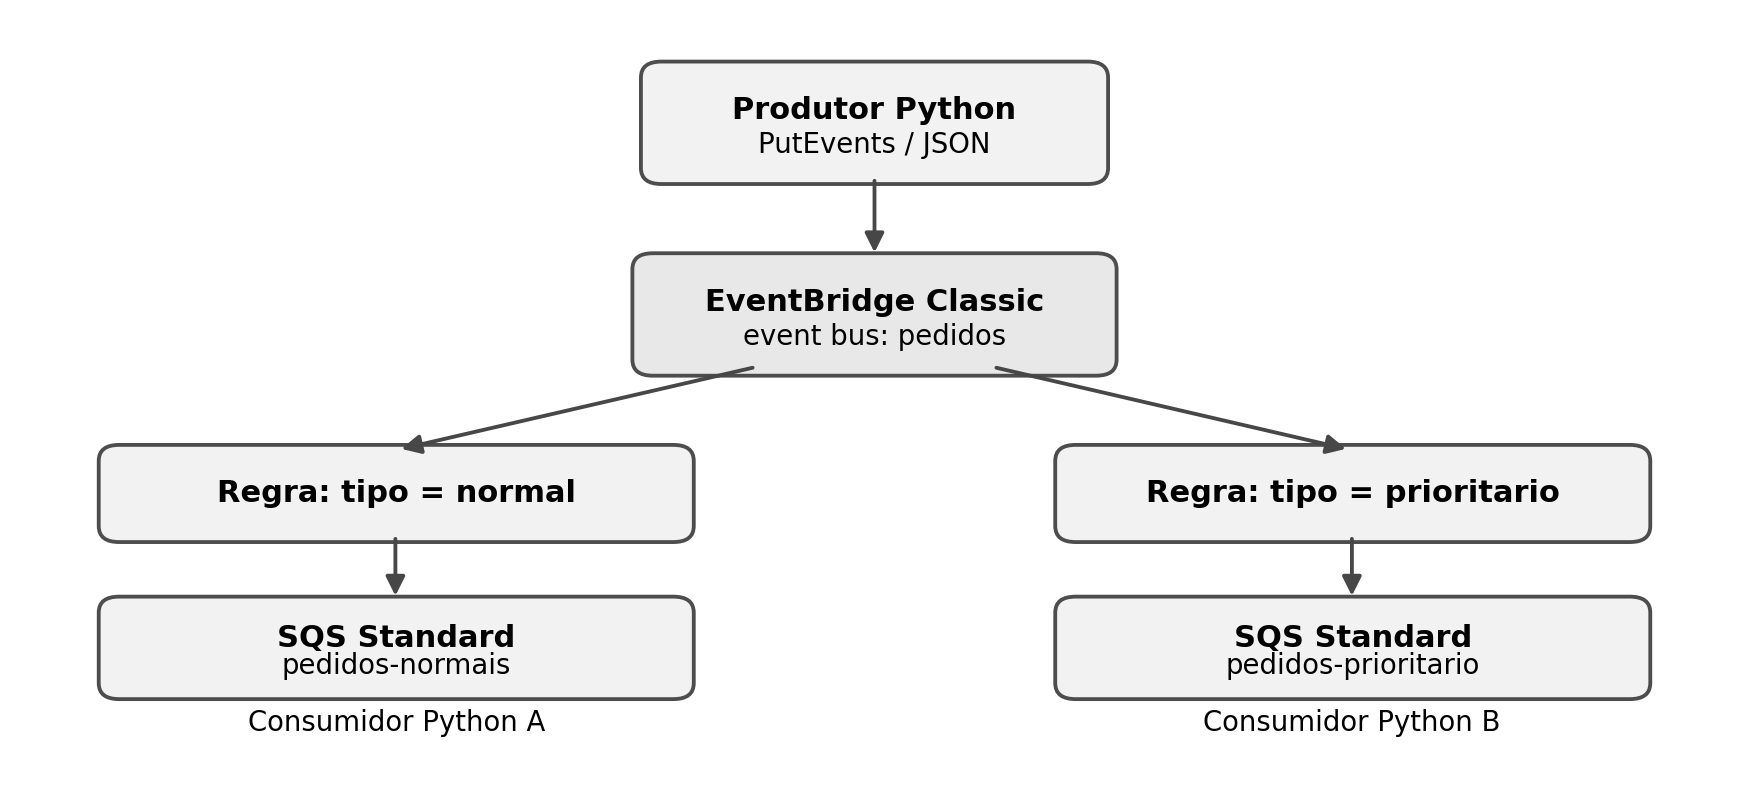
\includegraphics[width=.94\textwidth]{../figuras/arquitetura.png}
\caption{Arquitetura executada na AWS: barramento, filtragem por conteúdo,
filas SQS e consumidores independentes.}
\label{fig:arquitetura}
\end{figure}

O produtor envia lotes de até dez eventos por chamada. Dois consumidores
Python independentes, implementados com \emph{threads}, consultam suas filas
por \emph{long polling} de dois segundos, solicitando até dez mensagens por
chamada. Cada mensagem é registrada no CSV e excluída da fila após o registro.
O código de experimentação não recria recursos, não executa
\texttt{PurgeQueue} e não apaga mensagens de outras execuções: utiliza o
\texttt{run\_id} para distinguir os eventos pertencentes à coleta atual.

\section{Metodologia Experimental}
\subsection{Cenários e parâmetros}
O trabalho foi executado na AWS em 14 de novembro de 2026. A Tabela
\ref{tab:cenarios} descreve os cenários. Antes de cada ensaio, o programa
verifica por leituras sucessivas a profundidade aproximada das filas para
minimizar a mistura com mensagens antigas. Os ensaios de carga usam dois
consumidores simultâneos, já ativos quando a publicação começa.

\begin{table}[ht]
\centering
\caption{Cenários experimentais executados.}
\label{tab:cenarios}
\small
\setlength{\tabcolsep}{5pt}
\begin{tabular}{p{3.1cm}p{10.1cm}}
\toprule
Cenário & Procedimento \\
\midrule
Validação & Publicação de dois pedidos, um por fila. \\
Roteamento & 100 eventos válidos e dez com tipo \texttt{desconhecido}. \\
Carga & Cinco repetições por volume: 100, 500 e 1.000 eventos válidos. \\
Indisponibilidade & Publicação de 100 eventos sem consumidores ativos;
 espera de dez segundos e reativação dos consumidores. \\
\bottomrule
\end{tabular}
\end{table}

Os eventos válidos foram divididos igualmente entre as duas filas. Cada
repetição recebe \texttt{run\_id} exclusivo, e cada evento, um
\texttt{evento\_id} distinto. Os eventos inválidos do teste de roteamento
não correspondem a nenhuma das regras e, portanto, não devem ser observados
nas filas monitoradas. Em todos os ensaios, o programa registra envios,
recebimentos, erros e métricas consolidadas em arquivos CSV.

O cenário de indisponibilidade representa \emph{ausência de consumidores
antes da publicação}: os 100 eventos são publicados, os consumidores
permanecem desligados durante dez segundos e, em seguida, são iniciados.
Esse ensaio testa retenção e recuperação no SQS, e não a queda abrupta de um
processador durante a execução de uma tarefa.

\subsection{Métricas e cálculos}
O instante de envio é gerado imediatamente antes da chamada
\texttt{PutEvents} que inclui o evento, e o de recebimento é gerado após
\texttt{ReceiveMessage} retornar a mensagem ao consumidor. Para o evento
\(i\), define-se a latência observada:
\begin{equation}
L_i=t_{\text{recebimento},i}-t_{\text{envio},i}.
\end{equation}
Os dois \emph{timestamps} são medidos no mesmo CloudShell, mas o intervalo
inclui publicação, rede, EventBridge, fila, consultas SQS e escalonamento do
consumidor. Portanto, não é a latência interna do EventBridge. Média, mediana
e p95 de cada carga são calculados sobre todas as latências individuais do
volume (cinco repetições agregadas); a média da vazão é calculada entre
repetições.

A vazão observada por execução é definida como
\begin{equation}
V=\frac{N_{\text{IDs únicos corretos}}}
{t_{\text{último recebimento}}-t_{\text{primeiro envio}}}.
\end{equation}
A taxa de entrega correta, entre os eventos aceitos com destino esperado, é
\begin{equation}
T_c=\frac{N_{\text{IDs únicos na fila esperada}}}
{N_{\text{IDs aceitos com destino esperado}}}\times100\%.
\end{equation}
Também são contados IDs faltantes, entregas na fila incorreta, recebimentos
duplicados, erros de consumo e falhas na exclusão das mensagens. No cenário
de indisponibilidade, o tempo de recuperação é medido pelo próprio programa
desde a reativação dos consumidores até detectar os 100 IDs esperados. O
programa também coleta a profundidade aproximada das filas por meio de
\texttt{GetQueueAttributes}; esses contadores não são uma medição exata em
tempo real \cite{aws-sqs-metricas}.

\section{Resultados e Discussão}
\subsection{Roteamento funcional}
Foram realizadas 18 execuções completas: uma validação inicial, um ensaio
de roteamento, quinze execuções de carga e um ensaio de indisponibilidade.
No total, \textbf{8.212 eventos} foram aceitos pela API, dos quais 8.202
possuíam destino esperado. Todos os 8.202 foram registrados nas filas
corretas, sem faltantes, roteamentos incorretos ou duplicações detectadas
nas janelas observadas. Os dez eventos com tipo \texttt{desconhecido} não
foram observados nas duas filas. As 8.202 exclusões registradas ocorreram
com sucesso.

Esse resultado demonstra a correção funcional do roteamento dentro dos
ensaios realizados. Não significa que a plataforma garanta entrega
\emph{exactly-once}: o SQS Standard tem semântica \emph{at-least-once}
e não assegura ordenação estrita \cite{aws-sqs-standard}.

\subsection{Latência e vazão nas diferentes cargas}
A Tabela~\ref{tab:desempenho} sintetiza os resultados dos 8.000 eventos de
carga. Os percentis foram recalculados a partir dos registros individuais,
em vez de se obter uma média dos cinco p95 de cada carga.

\begin{table}[ht]
\centering
\caption{Métricas dos ensaios de carga (cinco repetições por volume).}
\label{tab:desempenho}
\small
\setlength{\tabcolsep}{4pt}
\begin{tabular}{rrrrrr}
\toprule
Eventos/ensaio & Recebidos & Média (s) & Mediana (s) & p95 (s) & Vazão (ev/s) \\
\midrule
100 & 500 & 1,326 & 0,411 & 4,434 & 20,71 \\
500 & 2.500 & 9,086 & 1,977 & 35,619 & 33,16 \\
1.000 & 5.000 & 15,808 & 5,863 & 52,562 & 33,04 \\
\bottomrule
\end{tabular}
\end{table}

A média agregada cresceu de 1,326~s para 9,086~s e 15,808~s conforme o
volume aumentou. Os p95 globais foram 4,434~s, 35,619~s e 52,562~s,
respectivamente. A Figura~\ref{fig:distribuicao} apresenta as distribuições
individuais (hastes entre p5 e p95) e os respectivos p95 globais.

\begin{figure}[ht]
\centering
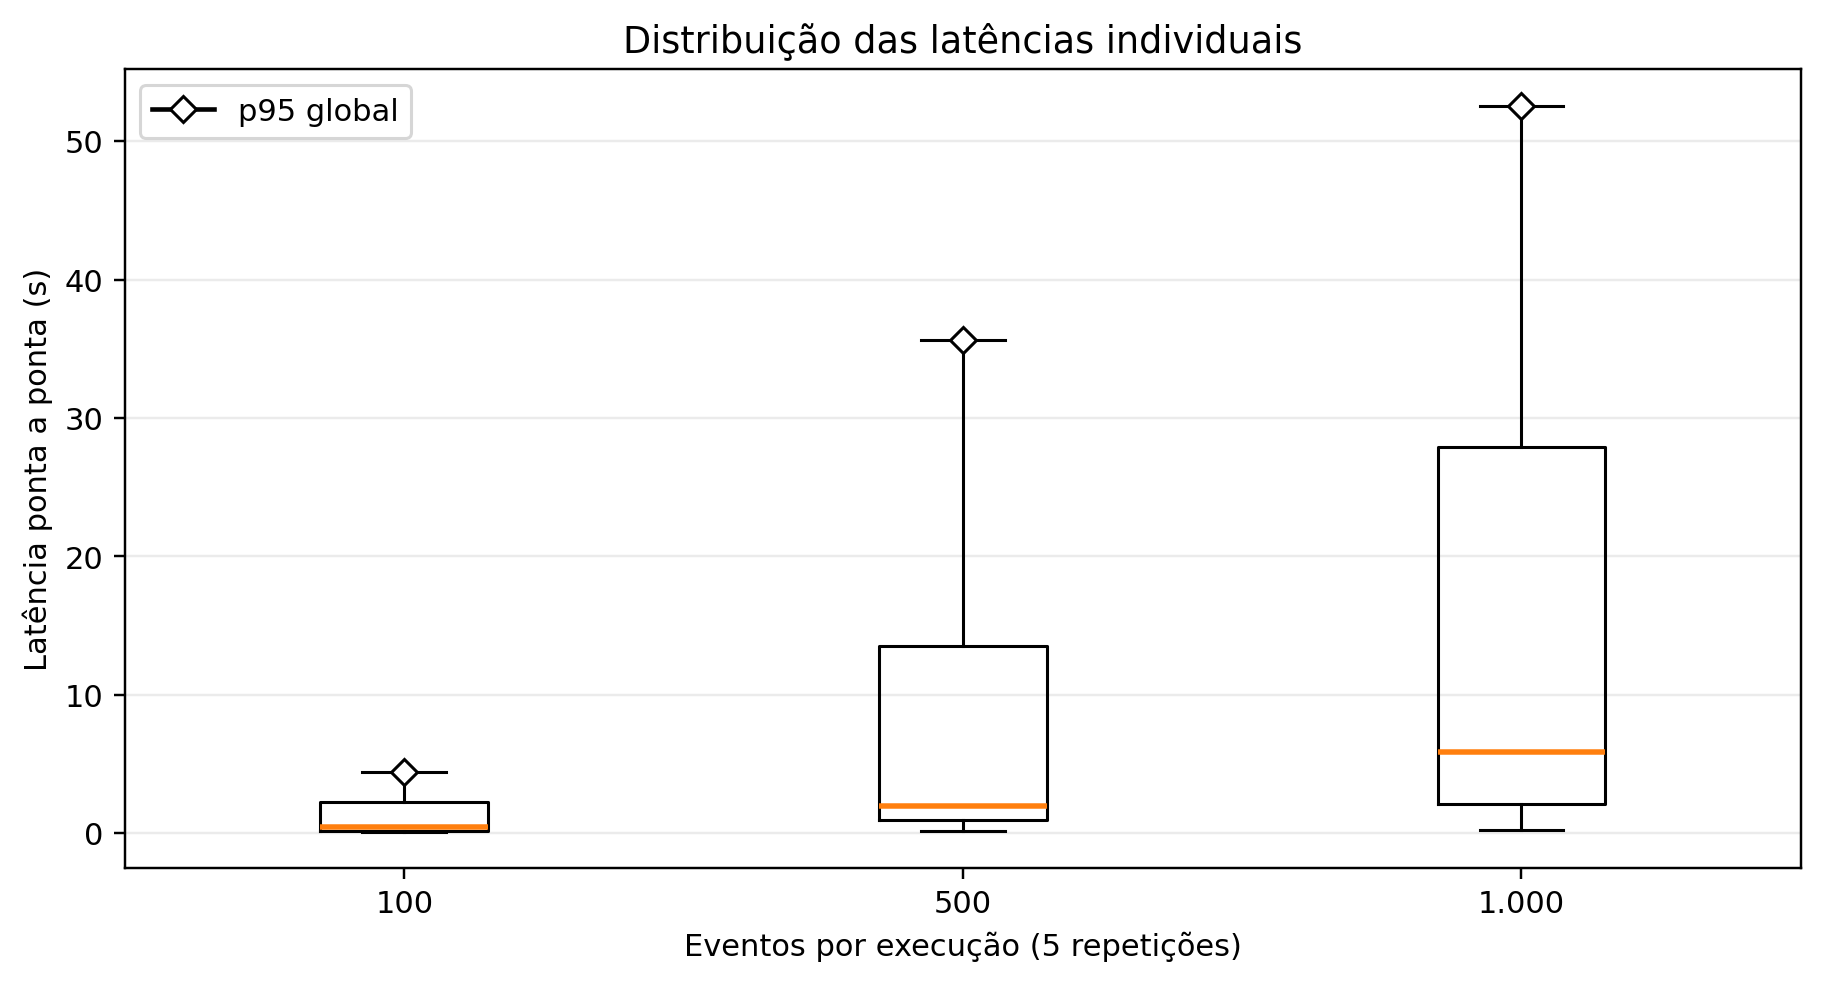
\includegraphics[width=.80\textwidth]{../figuras/distribuicao_latencia.png}
\caption{Distribuições individuais das latências por volume e percentil 95
calculado sobre todas as mensagens de cada carga.}
\label{fig:distribuicao}
\end{figure}

A tendência agregada encobre importante variabilidade entre execuções.
Nos ensaios de 500 eventos, três repetições apresentaram latência média
inferior a 2~s, enquanto duas atingiram 21,160~s e 19,240~s. Em 1.000
eventos, a média variou de 2,760~s a 33,833~s, com desvio padrão amostral
de 13,878~s entre as médias das cinco execuções. A Figura
\ref{fig:repeticoes} explicita essa dispersão.

\begin{figure}[ht]
\centering
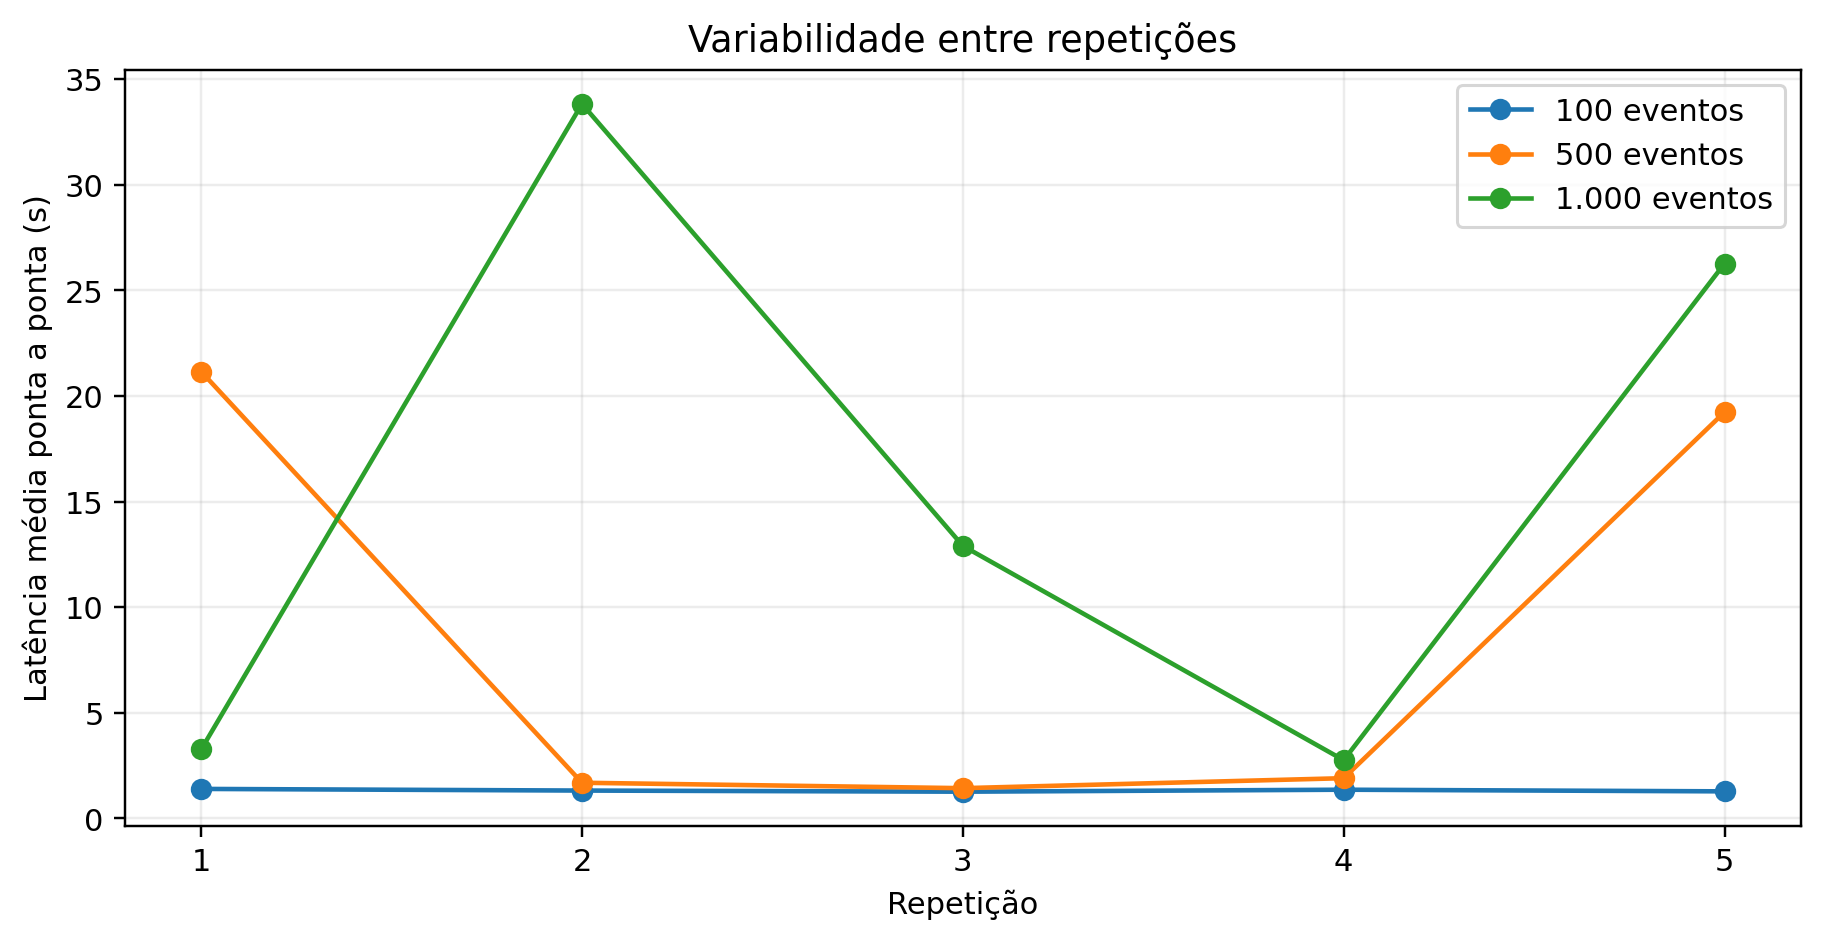
\includegraphics[width=.80\textwidth]{../figuras/variabilidade_repeticoes.png}
\caption{Latência média observada nas cinco repetições de cada carga.}
\label{fig:repeticoes}
\end{figure}

A vazão média entre execuções foi 20,71, 33,16 e 33,04 eventos/s para as
cargas de 100, 500 e 1.000 eventos, respectivamente. Nas cargas de 500 e
1.000, a vazão variou, respectivamente, entre 8,28--55,28 e
8,59--73,23 eventos/s. A duração da publicação variou de 1,144 a
27,086~s para 500 eventos e de 2,165 a 63,202~s para 1.000 eventos.
Essa variabilidade impede atribuir toda a diferença de latência ao
EventBridge: parte do tempo pode estar associada ao produtor, à API, à
rede, à fila ou às consultas dos consumidores.

\subsection{Indisponibilidade e recuperação}
No experimento de indisponibilidade foram aceitos 100 eventos, com 50
pedidos normais e 50 prioritários. Após a publicação, os consumidores
permaneceram ausentes durante dez segundos. A retomada dos consumidores
resultou no recebimento correto dos \textbf{100 IDs esperados}, sem falhas,
duplicações observadas ou mensagens na fila incorreta. O tempo de
recuperação calculado pelo script desde a reativação até a detecção do
recebimento completo foi \textbf{11,679~s}. A latência ponta a ponta média
do cenário foi 15,764~s, com p95 de 21,657~s; esses valores incluem a
pausa imposta ao processamento e não são diretamente comparáveis aos
ensaios de carga com consumidores continuamente ativos.

\begin{figure}[ht]
\centering
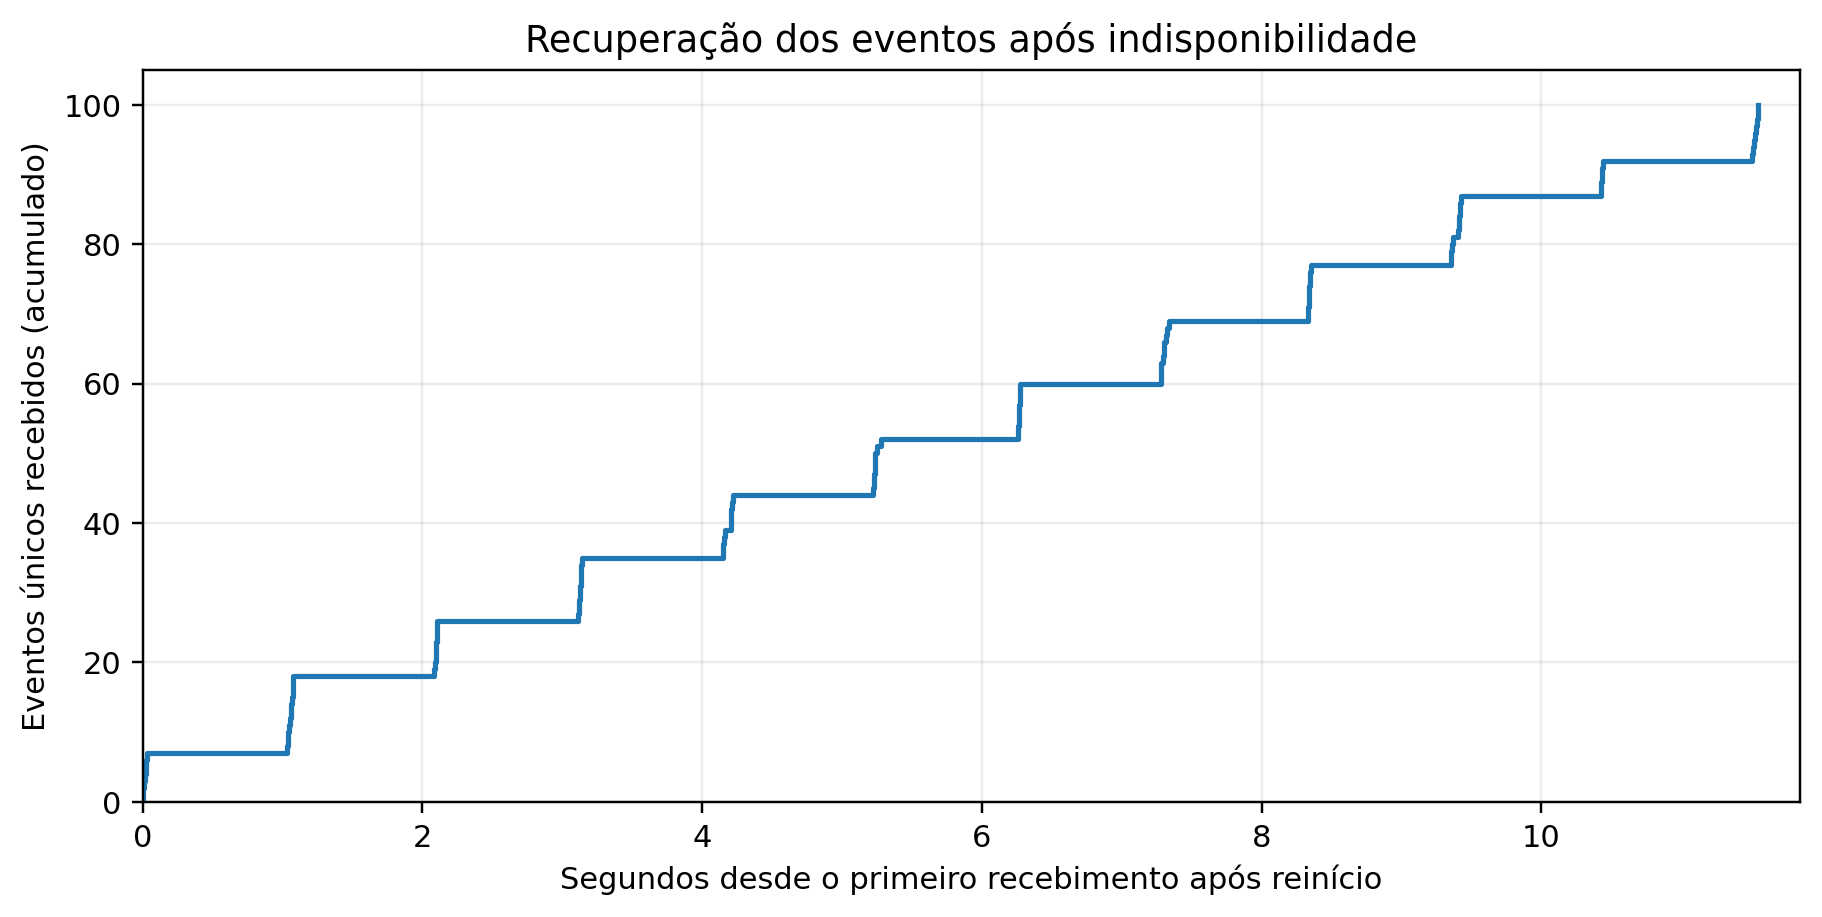
\includegraphics[width=.80\textwidth]{../figuras/recuperacao_acumulada.png}
\caption{Recebimento acumulado dos 100 eventos após a retomada; o eixo
horizontal começa no primeiro recebimento registrado.}
\label{fig:recuperacao}
\end{figure}

O programa registrou 100 mensagens como profundidade aproximada no
\emph{snapshot} interno utilizado antes do reinício; contudo, as amostras
consecutivas de profundidade das filas alternaram valores inconsistentes,
inclusive contagens que permaneceram positivas após a recepção confirmada
dos 100 eventos. Esses valores não são evidência de novas perdas, mas uma
limitação das métricas aproximadas do SQS em um intervalo curto. A Figura
\ref{fig:backlog} apresenta essas amostras, distinguindo-as dos registros
individualmente confirmados de recebimento \cite{aws-sqs-metricas}.

\begin{figure}[ht]
\centering
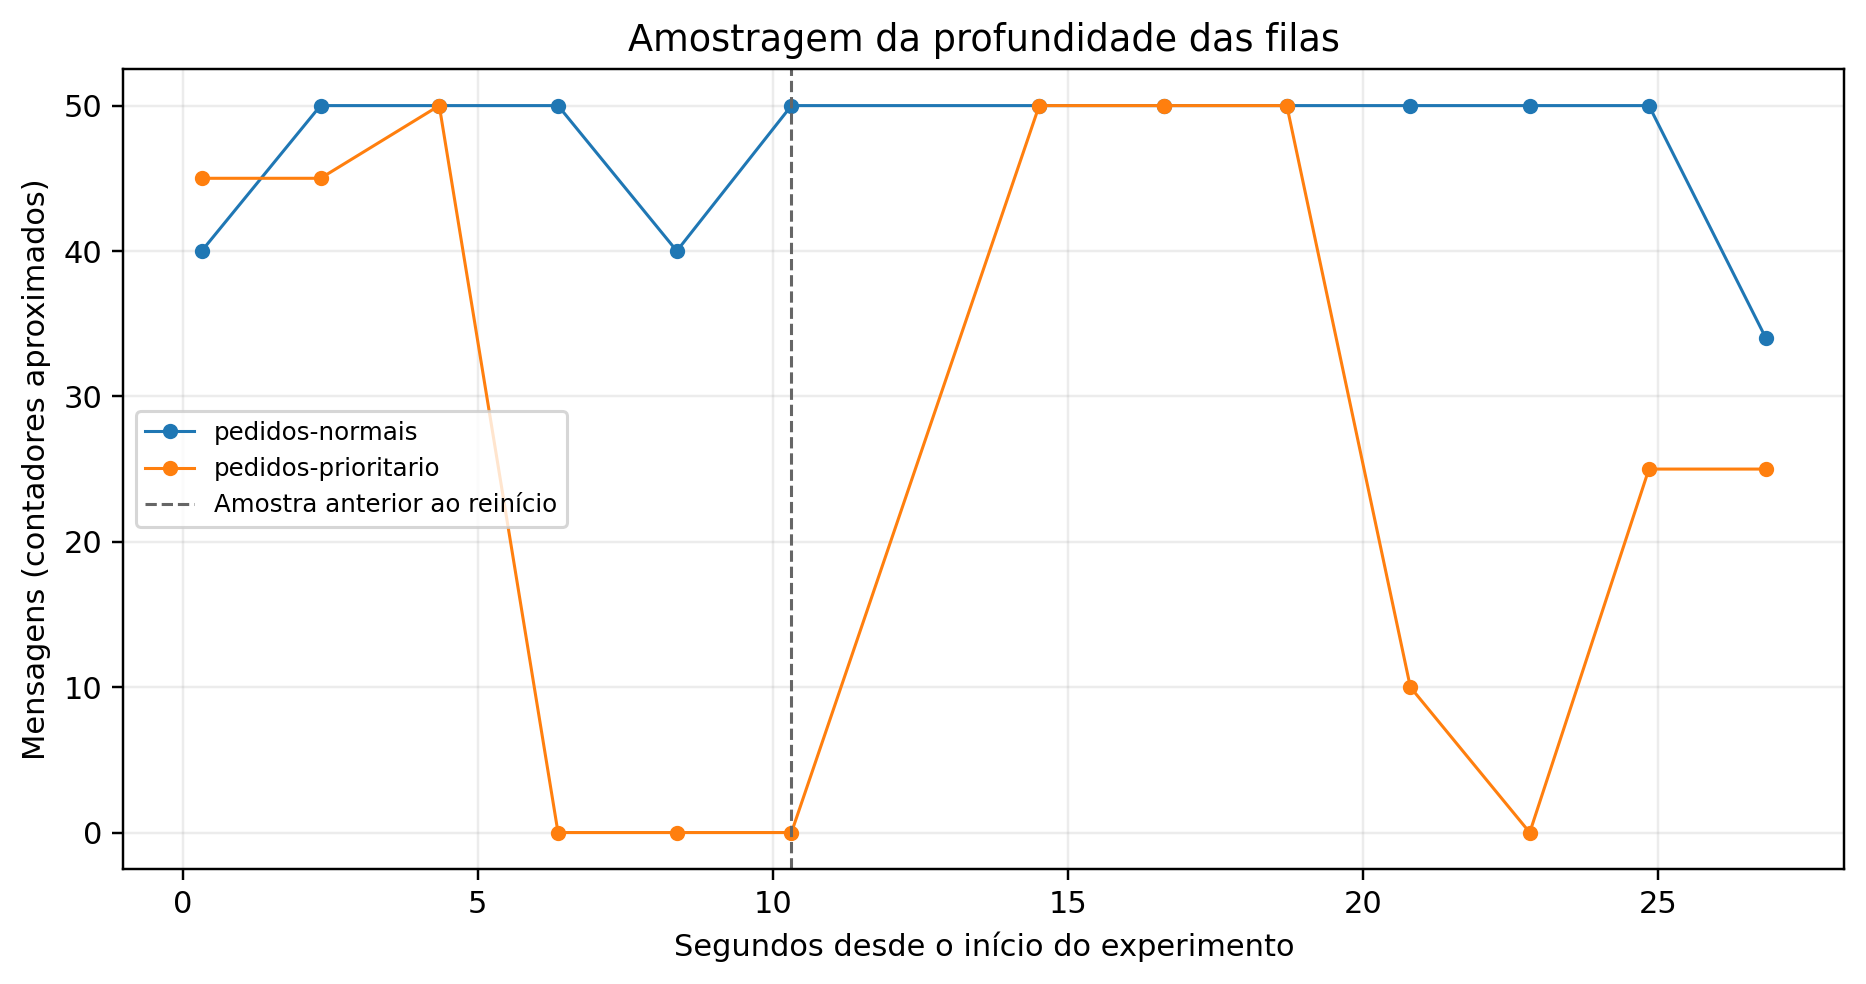
\includegraphics[width=.80\textwidth]{../figuras/backlog_aproximado.png}
\caption{Profundidade aproximada das filas por fase; oscilações mostram que
a contagem não equivale ao número exato de mensagens em cada instante.}
\label{fig:backlog}
\end{figure}

O ensaio evidencia o desacoplamento temporal viabilizado pela retenção no
SQS: o produtor conseguiu publicar os eventos enquanto os consumidores
estavam ausentes, e os consumidores os processaram depois. Essa retenção
é um comportamento do SQS, enquanto o EventBridge realizou o encaminhamento
por conteúdo; não se tratou de teste de política de retentativas do
EventBridge ou de uma fila de mensagens mortas.

\FloatBarrier
\section{Limitações e Ameaças à Validade}
O estudo se restringiu a uma única região da AWS e a um ambiente CloudShell
compartilhado. Não foram coletadas métricas de CPU, rede ou limites efetivos
do serviço, tampouco telemetria interna do EventBridge para isolar atrasos.
O envio em lotes, a política de \emph{polling} e a execução de dois
consumidores no mesmo ambiente impactam as medidas ponta a ponta. Os
payloads são pequenos e similares, sem experimentos de tamanho de mensagem.

As cargas foram executadas com ordem não aleatorizada, e cinco repetições
por volume não caracterizam estabilidade prolongada. Os testes registram
somente duplicações dentro da janela curta de observação, não garantindo
a ausência de recebimentos posteriores. As verificações de filas vazias
e as séries de \emph{backlog} dependem de contadores aproximados do SQS,
que oscilaram durante o ensaio. O experimento de indisponibilidade contém
uma única execução de 100 eventos e uma pausa programada; ele não avalia
falhas abruptas, falhas simultâneas das filas, nem políticas de DLQ.

A abordagem não compara diretamente EventBridge a REST, Kafka ou outros
middlewares sob a mesma carga. Qualquer afirmação de superioridade de
latência, custo operacional ou capacidade entre tecnologias exigiria uma
campanha experimental independente e com parâmetros equivalentes.

\section{Conclusão}
O protótipo confirmou o funcionamento de uma arquitetura orientada a eventos
com Amazon EventBridge Classic e Amazon SQS Standard, incluindo filtragem
por conteúdo, dois consumidores desacoplados e retenção durante uma
indisponibilidade simulada. Em 18 execuções, todos os 8.202 eventos com
destino esperado foram recebidos nas filas previstas, sem erros ou
duplicações detectados nas janelas de observação. Os ensaios de carga
produziram métricas de latência e vazão, mas revelaram alta dispersão
quando o volume cresceu, sem permitir atribuir causalmente os atrasos ao
EventBridge. No ensaio de indisponibilidade, os 100 eventos foram
recuperados após reativar os consumidores, com 11,679~s de recuperação
observada. O conjunto demonstra o potencial didático do middleware
orientado a eventos, ao mesmo tempo em que evidencia a necessidade de
métodos controlados e telemetria adicional para afirmações sobre desempenho
de produção.

\begin{thebibliography}{99}
\raggedright
\bibitem{tanenbaum2002} Tanenbaum, A. S. e van Steen, M. (2002).
\emph{Distributed Systems: Principles and Paradigms}. Prentice Hall.
\bibitem{hohpe2003} Hohpe, G. e Woolf, B. (2003).
\emph{Enterprise Integration Patterns: Designing, Building, and Deploying Messaging Solutions}.
Addison-Wesley.
\bibitem{aws-eb} Amazon Web Services. \emph{What Is Amazon EventBridge?}.
\url{https://docs.aws.amazon.com/eventbridge/latest/userguide/eb-what-is.html}.
Acesso em: 14 nov. 2026.
\bibitem{aws-permissoes} Amazon Web Services. \emph{Using Resource-Based Policies for Amazon EventBridge}.
\url{https://docs.aws.amazon.com/eventbridge/latest/userguide/eb-use-resource-based.html}.
Acesso em: 14 nov. 2026.
\bibitem{aws-sqs-standard} Amazon Web Services. \emph{Amazon SQS Standard Queues}.
\url{https://docs.aws.amazon.com/AWSSimpleQueueService/latest/SQSDeveloperGuide/standard-queues.html}.
Acesso em: 14 nov. 2026.
\bibitem{aws-sqs-metricas} Amazon Web Services. \emph{Available CloudWatch Metrics for Amazon SQS}.
\url{https://docs.aws.amazon.com/AWSSimpleQueueService/latest/SQSDeveloperGuide/sqs-available-cloudwatch-metrics.html}.
Acesso em: 14 nov. 2026.
\end{thebibliography}
\end{document}
